\section{Tecniche di Data Augmentation}

La data augmentation comprende una vasta gamma di tecniche che trasformano le immagini esistenti per generare nuovi esempi di addestramento.

\subsection{Tecniche Base di Data Augmentation}
Queste tecniche mirano a incrementare la variabilità dei dati di addestramento attraverso modifiche semplici e intuitive, permettendo al modello di imparare a riconoscere gli oggetti in una varietà di condizioni e configurazioni.

\subsubsection{Trasformazioni Geometriche}
Le trasformazioni geometriche sono tecniche che alterano la posizione o la forma degli oggetti nell'immagine senza modificarne il contenuto. Queste tecniche sono utili per rendere i modelli di computer vision più robusti alle variazioni spaziali.

\begin{itemize}
  \item \textbf{Rotazione}: ruota l'immagine di un determinato angolo - aiuta il modello a riconoscere oggetti indipendentemente dalla loro orientazione.
  \item \textbf{Traslazione}: sposta l'immagine lungo gli assi X e Y - aiuta il modello a riconoscere oggetti che potrebbero essere presenti in posizioni diverse nell'immagine.
  \item \textbf{Ritaglio}: seleziona una porzione dell'immagine originale - migliora la capacità del modello di identificare oggetti che possono essere solo parzialmente visibili.
  \item \textbf{Zoom}: ingrandimento o riduzione dell'immagine - aiuta il modello ad identificare oggetti a diverse scale.
  \item \textbf{Flip}: ribalta l'immagine orizzontalmente, verticalmente o entrambe - aiuta il modello a imparare che gli oggetti possono apparire in orientazioni diverse.
\end{itemize}

\begin{figure}[ht]
    \centering
    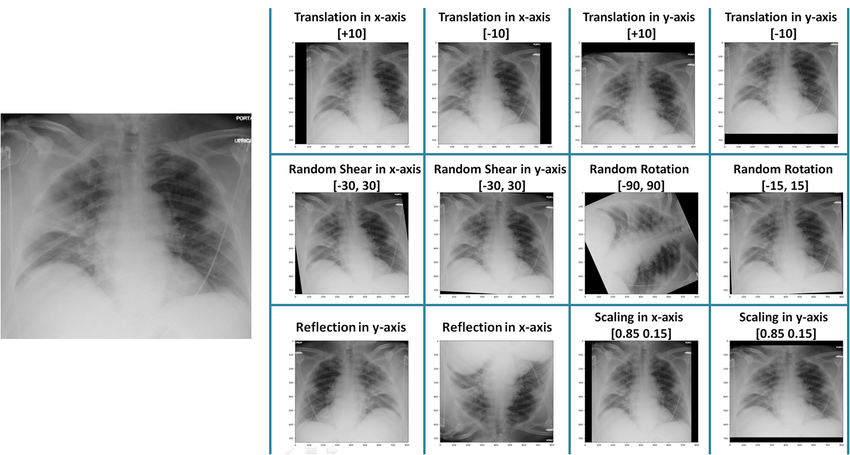
\includegraphics[width=0.9\textwidth]{files/capitoli/3-data-augmentation/assets/geometric-transformations.png}
    \caption{\label{fig:geometric-transformations}Esempi di trasformazioni geometriche applicate ad un'immagine X-ray\cite{34}}
\end{figure}

\subsubsection{Modifiche dei Colori}
Le modifiche dei colori alterano i valori cromatici nell'immagine, aiutando il modello a riconoscere gli oggetti sotto diverse condizioni di illuminazione e colore.

Possiamo andare a modificare:
\begin{itemize}
  \item \textbf{Luminosità}: migliora la capacità del modello di adattarsi a condizioni di luce diverse
  \item \textbf{Saturazione}: aiuta il modello a riconoscere gli oggetti indipendentemente dall'intensità dei colori
  \item \textbf{Contrasto}: permette al modello di distinguere meglio gli oggetti in base alle differenze di luminosità
  \item \textbf{Colore}: aiuta il modello a riconoscere gli oggetti indipendentemente dalle condizioni cromatiche.
\end{itemize}

\begin{figure}[ht]
    \centering
    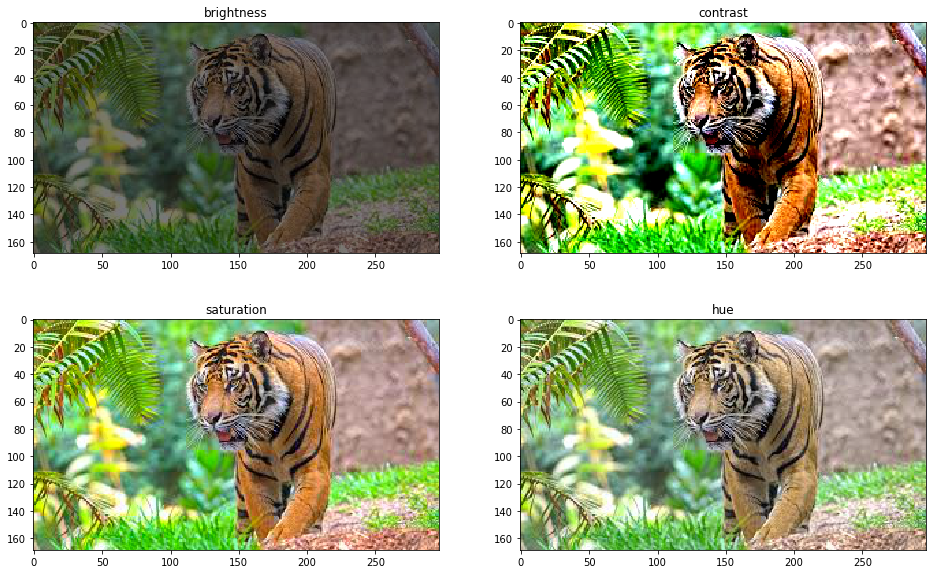
\includegraphics[width=0.8\textwidth]{files/capitoli/3-data-augmentation/assets/color-transformations.png}
    \caption{\label{fig:color-transformations}Esempi di trasformazioni di colore applicate ad una foto\cite{35}}
\end{figure}

\subsubsection{Distorsioni e Rumore}
Le distorsioni e l'aggiunta di rumore all'immagine possono migliorare la robustezza del modello, aiutandolo a imparare a riconoscere gli oggetti anche in condizioni non ideali o con interferenze.

\begin{itemize}
  \item \textbf{Distorsione Elastica}: introduce deformazioni locali all'immagine, aumentando la varietà dei pattern geometrici presenti nei dati di addestramento.
  \item \textbf{Aggiunta di Rumore Gaussiano}: introduce variazioni casuali simili al rumore nei sensori delle fotocamere, migliorando la capacità del modello di distinguere dettagli sottili e rendendolo più robusto contro i disturbi.
  \item \textbf{Aggiunta di Rumore Salt-and-Pepper}: simula interferenze come granelli di polvere o artefatti minori, rendendo il modello più robusto rispetto alle imperfezioni dell'immagine.
  \item \textbf{Blur}: sfoca l'immagine simulando condizioni di scarsa qualità, migliorando la capacità del modello di riconoscere oggetti in condizioni di bassa definizione o in movimento.
  \item \textbf{Distorsione da Lente}: introduce distorsioni ottiche simili a quelle causate da lenti fotografiche, migliorando la capacità del modello di adattarsi a variazioni nelle proporzioni degli oggetti.
\end{itemize}

\vspace{1cm}

\begin{figure}[ht]
    \centering
    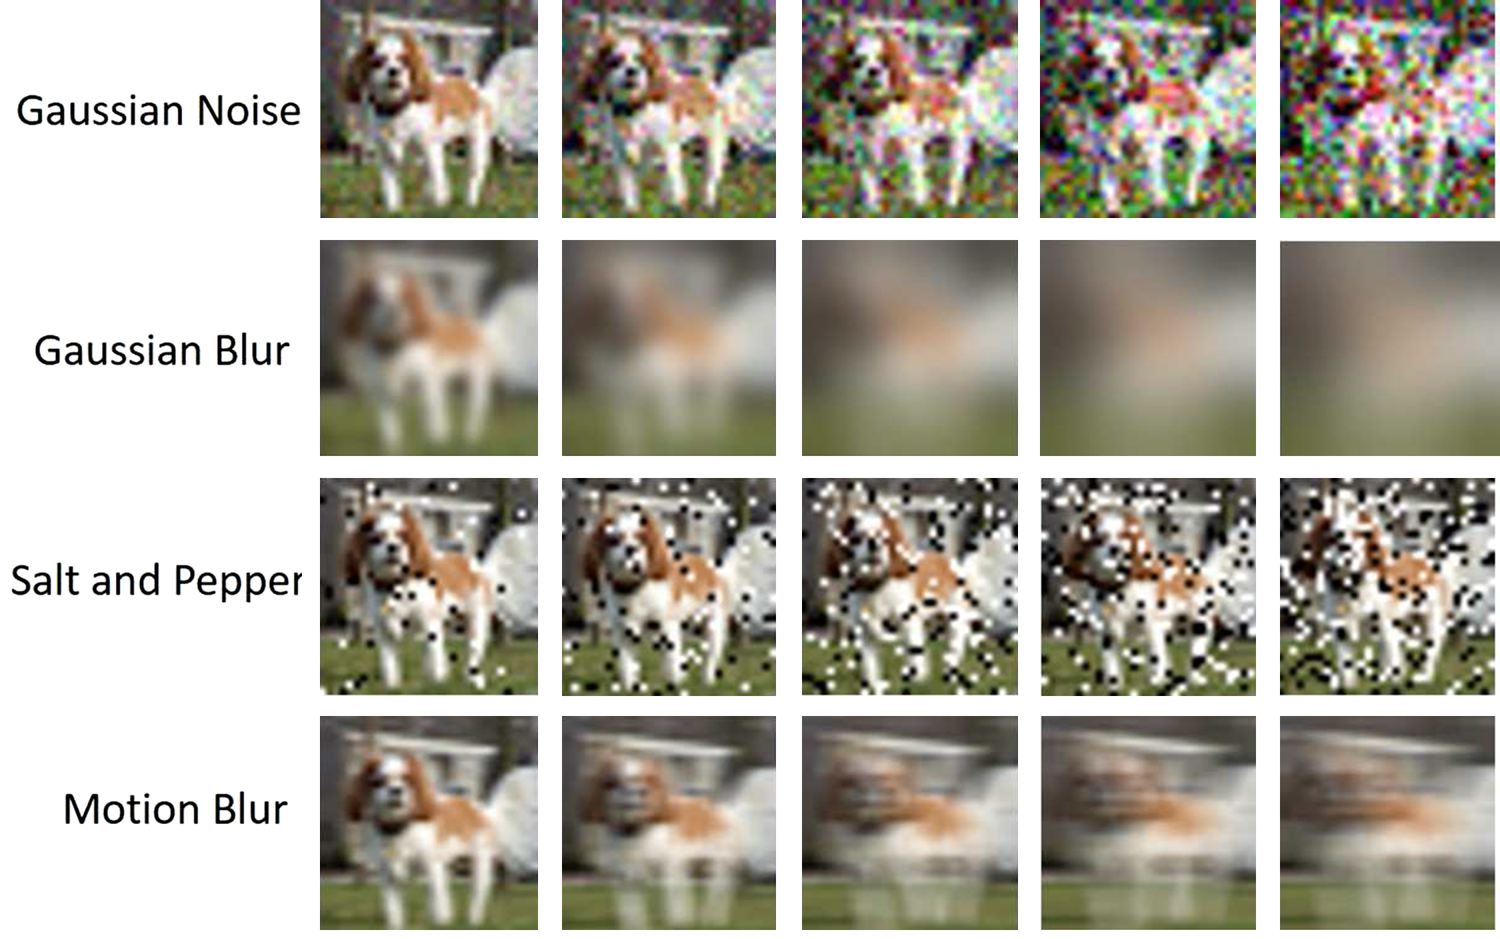
\includegraphics[width=0.8\textwidth]{files/capitoli/3-data-augmentation/assets/distortion-noise.png}
    \caption{\label{fig:distortion-noise}Esempi di distorsioni ed aggiunte di rumore\cite{36}}
\end{figure}

\newpage

\subsection{Tecniche Avanzate di Data Augmentation}
Le tecniche avanzate di data augmentation vanno oltre le trasformazioni geometriche ed i cambiamenti di colore, introducendo strategie più complesse per migliorare le prestazioni dei modelli. Queste tecniche sono progettate per generare dati sintetici più diversificati e realistici, migliorando così la capacità del modello di generalizzare su dati non visti durante l'addestramento.

\subsubsection{Augmentation tramite GAN}
L'Augmentation tramite Generative Adversarial Networks (GAN) è una tecnica che utilizza reti neurali generative e discriminative per generare dati sintetici ad alta fedeltà. Questi modelli apprendono la distribuzione dei dati di input e generano esempi che sono coerenti con tale distribuzione. 

\vspace{0.5cm}

\begin{figure}[ht]
    \centering
    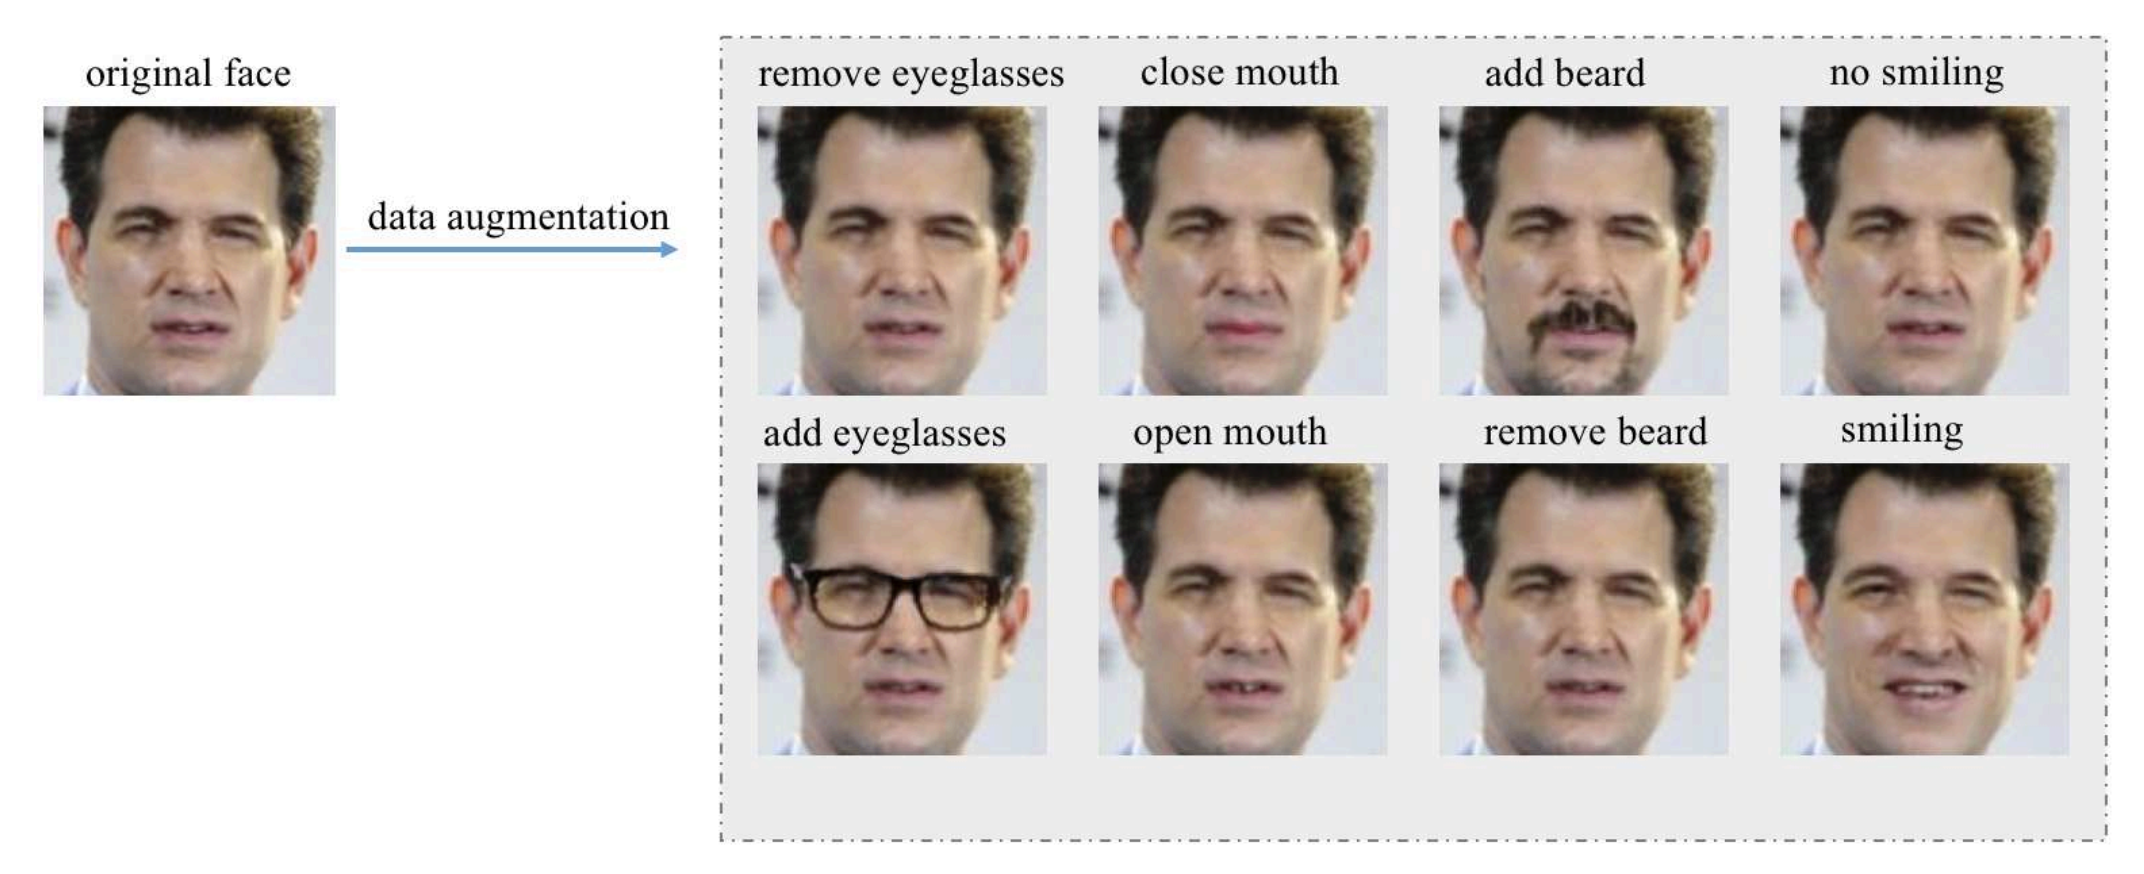
\includegraphics[width=0.9\textwidth]{files/capitoli/3-data-augmentation/assets/gan-augmentation.png}
    \caption{\label{fig:gan-augmentatione}Esempi di immagini generate tramite GAN\cite{37}}
\end{figure}

\newpage

\subsubsection{Mixup, Cutout e Cutmix}
Mixup è una tecnica di data augmentation che mescola coppie di campioni di addestramento per creare nuovi esempi. Questa tecnica combina le immagini e le etichette dei campioni originali per creare nuove istanze durante l'addestramento. D'altra parte, Cutout è una tecnica che consiste nel mascherare casualmente parti delle immagini di addestramento, incoraggiando il modello a focalizzarsi su caratteristiche meno sensibili al rumore. Infine CutMix è una tecnica che unisce le precedenti, ritagliando regioni delle immagini come nel Cutout, ma andandoci ad incollare pezzi di altri esempi. Questa tecnica forza il modello a generalizzare meglio, rendendolo robusto alle distorsioni localizzate e migliorando la sua capacità di rilevare e classificare oggetti anche in presenza di parziali occlusioni.

\vspace{0.5cm}

\begin{figure}[ht]
    \centering
    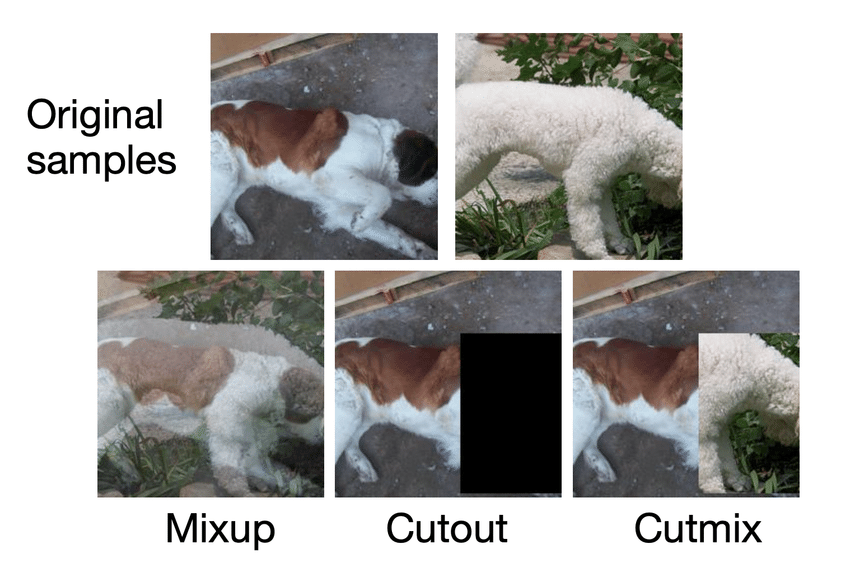
\includegraphics[width=0.8\textwidth]{files/capitoli/3-data-augmentation/assets/mixup-cutout-cutmix.png}
    \caption{\label{fig:gan-augmentatione}Esempi di Mixup, Cutout e Cutmix\cite{38}}
\end{figure}

\newpage